% This must be in the first 5 lines to tell arXiv to use pdfLaTeX, which is strongly recommended.
\pdfoutput=1
% In particular, the hyperref package requires pdfLaTeX in order to break URLs across lines.

\documentclass[11pt]{article}

% Remove the "review" option to generate the final version.
\usepackage[]{acl}

% Standard package includes
\usepackage{times}
\usepackage{latexsym}

\usepackage{microtype}
\usepackage{wrapfig,lipsum,booktabs}
\usepackage{amsmath,amssymb} % define this before the line numbering.
\usepackage{subcaption}
\usepackage{color}
\usepackage{tikz}
\usepackage{graphicx}
\usepackage{soul}
\usepackage{comment}
% following 3 packages for forcing the caption at the top
% \usepackage{float}
\usepackage{floatrow}
% \floatstyle{plaintop}
% \restylefloat{table}
\usepackage{todonotes}
\usepackage{url}
\usepackage{hyperref}
\usepackage{blindtext}
\usepackage{enumitem}
\usepackage{amssymb}
\usepackage{multirow}
\usepackage{arydshln}

% For proper rendering and hyphenation of words containing Latin characters (including in bib files)
\usepackage[T1]{fontenc}
% For Vietnamese characters
% \usepackage[T5]{fontenc}
% See https://www.latex-project.org/help/documentation/encguide.pdf for other character sets

% This assumes your files are encoded as UTF8
\usepackage[utf8]{inputenc}
\newcommand{\dataset}{\textcolor{black}{\texttt{HVVMemes}}}
% \newcommand{\dataset}{\texttt{RIME}}
\newcommand{\harmeme}{\texttt{HarMeme}}
\newcommand{\model}{\texttt{MeRaiM}}
% \definecolor{deepgreen}{rgb}{0.0, 0.5, 0.0}
\definecolor{deepgreen}{rgb}{0.01, 0.75, 0.24}

% This is not strictly necessary, and may be commented out,
% but it will improve the layout of the manuscript,
% and will typically save some space.
\usepackage{microtype}

% If the title and author information does not fit in the area allocated, uncomment the following
%
%\setlength\titlebox{<dim>}
%
% and set <dim> to something 5cm or larger.

\title{Findings of the CONSTRAINT 2022 Shared Task\\ on Detecting the Hero, the Villain, and the Victim in Memes}

% Author information can be set in various styles:
\author{Shivam Sharma$^{1,3}$, Tharun Suresh$^1$, Atharva Kulkarni$^1$, Himanshi Mathur$^{1}$,\\ \textbf{Preslav Nakov$^2$, Md. Shad Akhtar$^1$, Tanmoy Chakraborty$^1$}\\
  $^1$Indraprastha Institute of Information Technology - Delhi, India  \\
  $^2$Qatar Computing Research Institute, HBKU, Doha, Qatar \\
  $^3$Wipro AI Labs, India\\
  \small\texttt{\{shivams, tharun20119, atharvak, himanshi18037, shad.akhtar, tanmoy\}@iiitd.ac.in}\\\small\texttt{pnakov@hbku.edu.qa}}

% For several authors from the same institution:
% \author{Shivam Sharma \and Tharun Suresh \and Atharva Kulkarni \and Himanshi Mathur \and Preslav Nakov \and Md. Shad Akhtar \and Tanmoy Chakraborty\\
%         Indraprastha Institute of Information Technology - Delhi }
%         \\ ... \\ Address line}
% if the names do not fit well on one line use
%         Author 1 \\ {\bf Author 2} \\ ... \\ {\bf Author n} \\
% For authors from different institutions:
% \author{Author 1 \\ Address line \\  ... \\ Address line
%         \And  ... \And
%         Author n \\ Address line \\ ... \\ Address line}
% To start a seperate ``row'' of authors use \AND, as in
% \author{Author 1 \\ Address line \\  ... \\ Address line
%         \AND
%         Author 2 \\ Address line \\ ... \\ Address line \And
%         Author 3 \\ Address line \\ ... \\ Address line}

% \author{First Author \\
%   Affiliation / Address line 1 \\
%   Affiliation / Address line 2 \\
%   Affiliation / Address line 3 \\
%   \texttt{email@domain} \\\And
%   Second Author \\
%   Affiliation / Address line 1 \\
%   Affiliation / Address line 2 \\
%   Affiliation / Address line 3 \\
%   \texttt{email@domain} \\}

\begin{document}
\maketitle
\begin{abstract}
% A frequent problem in meme comprehension lies in interpreting its broader context and its entities. Real-world multimedia applications involving memes often require knowledge of the entities illustrated in them and their interaction with one another. As a result, decipher the connotations behind the entities in a meme. In more nuanced terms, determining the victimizing, glorifying, and vilifying intentions embedded in meme entities seems plausible to explicate their connotations. We address this problem by proposing the novel task of \textit{role identification of entities in memes} -- which entity in a meme is the `hero', the `villain', and the `victim'. To this end, we curate \dataset, a novel meme dataset containing entities and their associated roles -- hero, villain, victim, others. Formulating the problem a role labelling task, we benchmark \dataset\ with numerous unimodal and multimodal baselines, therefore, validating the feasibility of the task. Furthermore, we design \model, a simple yet potent multimodal framework that interpolates entity-based contextual information in the multimodal representations. Empirical investigations attest to the model's efficacy in role identification of meme entities, with a $4\%$ boost over baselines for the macro-F1 score. Through rigorous qualitative and quantitative scrutiny, we shed light on including contextual information for meme analysis. We also release our detailed annotation guidelines for public use.

We present the findings of the shared task at the CONSTRAINT 2022 Workshop: \textit{Hero, Villain, and Victim: Dissecting harmful memes for Semantic role labeling of entities}. The task aims to delve deeper into the domain of meme comprehension by deciphering the connotations behind the entities present in a meme. In more nuanced terms, the shared task focuses on determining the victimizing, glorifying, and vilifying intentions embedded in meme entities to explicate their connotations. To this end, we curate \dataset, a novel meme dataset of about 7000 memes spanning the domains of COVID-19 and US Politics, each containing entities and their associated roles: \emph{hero}, \emph{villain}, \emph{victim}, or \emph{none}. The shared task attracted 105 participants, but eventually only 6 submissions were made. The successful submissions majorly relied on an ensemble of language and multimodal models. The best submission achieved an F1-score of 58.67.
\end{abstract}

\section{Introduction}

In recent years, the unwarranted spread of misinformation \cite{wu2019misinformation}, propaganda \cite{da-san-martino-etal-2020-semeval}, fake news \cite{ALDWAIRI2018215}, hate speech \cite{MacAvaney2019Hate}, and other harmful content has plagued social media platforms. Lately, the multimodal medium of \textit{memes} has materialized as a powerful means to disseminate such malicious content due to their ability to circumvent censorship norms \cite{mina2014batman} and to their fast-spreading nature.\footnote{\url{https://blog.hubspot.com/marketing/visual-content-marketing-strategy}} Thus, with an aptly crafted combination of images and text, a seemingly na\"{i}ve meme can easily become a source of harmful information diffusion. As a result, exploring the noxious side of memes has become a pressing research topic \cite{sharma-etal-2020-semeval,pramanick-etal-2021-detecting}.

While meme analysis has been studied in a variety of contexts, such as hate speech \cite{zhou2021multimodal,kiela2020hateful} harmfulness \cite{pramanick-etal-2021-detecting,pramanick-etal-2021-momenta-multimodal}, emotions \cite{sharma-etal-2020-semeval}, misinformation \cite{zidani2021memes}, sarcasm \cite{kumar2019sarc}, and offensiveness \cite{suryawanshi-etal-2020-multimodal}, limited forays have been made on comprehending the role of the entities that make up a meme. Tackling this bottleneck, this shared task focuses on identifying the \textit{`hero'}, \textit{`villain'}, and \textit{`victim'} entities present in a meme. Given a meme and its entities, the task entails identifying the entities belonging to the classes of hero, villain, and victim. Such categorization of the entities in the meme helps assimilate the entity-specific connotation and their nature, attitudes, decisions, and demeanour. For instance, when the meme creators intend to spread misinformation and hatred towards minority communities or defame certain individuals, politicians, and organizations, they depict the associated entities negatively. Similarly, when the intention is to shed light on the deplorable state of certain entities or glorify their heroism, entities are cast as victims or heroes, respectively. 
% ----------------------------------------------------------------------------------------------------

\begin{figure*}[t!]
\centering
\scriptsize
% \fontsize{6}{6}\selectfont
% \subfloat[\label{fig:meme_cov_her}]{
% \begin{tabular}{|c|}
% \multicolumn{1}{c}{\includegraphics[width=0.25\textwidth, height=0.25\textwidth]{figures/meme_examples/covid_memes_2521_her.png}}\\ \cline{2-2}
%       \texttt{[\textcolor{red}{donald trump}]} \\
%      \cdashline{2-2}
%      -
%      \\ \cdashline{2-2}
%      \multirow{3}{11em}{\texttt{[\textcolor{blue}{barack obama, john f. kennedy, abraham lincoln}]}}\\ 
%      \\
%      \\
%      \cline{2-2}
% \end{tabular}
% }
% \subfloat[\label{fig:meme_cov_vil}]{
% \begin{tabular}{|c|}
%      \multicolumn{1}{c}{\includegraphics[width=0.25\textwidth, height=0.25\textwidth]{figures/meme_examples/covid_memes_2541_vil.png}}\\ \hline
%      \multirow{3}{11em}{\texttt{[\textcolor{red}{muslimist,mask, obamaist,comunist, socialist}]}} \\
%      \\
%      \\
%     %  &\\
%      \cdashline{1-1}
%      - \\ \cdashline{1-1}
%      -\\ 
%      \hline
% \end{tabular}
% }
\subfloat[\label{fig:meme_pol_her}]{
\begin{tabular}{|c|}
     \multicolumn{1}{c}{\includegraphics[width=0.25\textwidth, height=0.25\textwidth]{figures/meme_examples/covid_memes_2521_her.png}}\\ \hline
    %  \\
    %  &\\
    %  \cdashline{1-1}
    %  \\ \cdashline{1-1}
     \multirow{2}{19em}{\texttt{[\textcolor{blue}{Barack Obama, John F. Kennedy, Abraham Lincoln}]} \texttt{[\textcolor{red}{Donald Trump}]}} \\ 
     \\
    %  \\
     \hline
\end{tabular}
}
\subfloat[\label{fig:meme_pol_vil}]{
\begin{tabular}{|c|}
     \multicolumn{1}{c}{\includegraphics[width=0.25\textwidth, height=0.25\textwidth]{figures/meme_examples/memes_1769_vil.png}}\\ \hline
     \multirow{2}{19em}{\texttt{[\textcolor{red}{Green Party, Jill Stein}]}} \\
     \\
    %  \\
    %  &\\
    %  \cdashline{1-1}
    %  -\\ \cdashline{1-1}
    %  -\\ 
     \hline
\end{tabular}
}
\subfloat[\label{fig:meme_cov_vic}]{
\begin{tabular}{|c|}
     \multicolumn{1}{c}{\includegraphics[width=0.25\textwidth, height=0.25\textwidth]{figures/meme_examples/memes_5033_vic.png}}\\ \hline
    %  -\\
    %  &\\
    %  \cdashline{1-1}
     \multirow{2}{19em}{\texttt{[\textcolor{deepgreen}{Women, Poor, Minorities}]} \texttt{[\textcolor{red}{Republican Party}]}} \\
     \\
    %  \\
    %  \cdashline{1-1}
    %  -\\
     \hline
\end{tabular}
}
% \subfloat[\label{fig:meme_pol_vic}]{
% \begin{tabular}{|c|}
%      \multicolumn{1}{c}{\includegraphics[width=0.25\textwidth, height=0.25\textwidth]{figures/meme_examples/memes_5033_vic.png}}\\ \hline
%       \texttt{[\textcolor{red}{republican party}]}\\
%     %  &\\
%      \cdashline{1-1}
%      \multirow{3}{11em}{\texttt{[\textcolor{orange}{women, poor, minorities}]}} \\
%         \\
%         \\
%         \cdashline{1-1}
%      -\\ 
%      \hline
% \end{tabular}
% }
\caption{Examples of \texttt{\textcolor{blue}{heroes}}, \texttt{\textcolor{red}{villains}} and \texttt{\textcolor{deepgreen}{victims}}, as portrayed within memes.}
% \hl{We need labels for each subfigure - who is hero/villian/victim.}}
\label{fig:meme_hvv_eg}
\end{figure*}



% --------------------------------------------------------------------------------------------------------
Fig.~\ref{fig:meme_hvv_eg} depicts apt examples for hero, villain, and victim categorization of the entities in a meme. The meme in Fig.~\ref{fig:meme_pol_her} draws a comparison between Abraham Lincoln, John F. Kennedy, Barack Obama, and Donald Trump, in which the former three are expressed as \emph{heroes} while Donald Trump is characterized in a negative light, thus, making him a \emph{villain}. Along similar lines, Fig.~\ref{fig:meme_pol_vil} mocks Jill Stein and the Green Party as \emph{villains} for allegedly getting bribed by the rich people. Fig.~\ref{fig:meme_cov_vic}, on the other hand, frames the Republican Party as a \emph{villain}, for their inconsiderate views on the poor, minorities, and women, thus, making them the \emph{victims}. In conclusion, through depictions of heroism, villainy, and victimization, memes act as an appealing means to spread entity-relevant information and opinions.

While some studies have sought to identify memes' harmfulness and the respective targeted categories \cite{pramanick-etal-2021-detecting,pramanick-etal-2021-momenta-multimodal}, none of them scrutinize the entity's connotation, let alone categorizing them as hero, villain, and victim. This shared task aims to address this quandary and foster further research in this direction. Thus, we release \dataset, a meme dataset peculiar to our task, with about $7000$ memes spanning COVID-19 and US Politics domains. Each contains entities and associated roles -- hero, villain, victim and none. The shared task amassed a total of $105$ participants with $6$ final submissions, most of which opted for fine-tuning pre-trained language and multimodal models and ensemble techniques. The best submission scored an F1-score of $58.67$. We elaborate on some of the top submissions in section~\ref{sec:partres}.

Despite the rising body of research in meme analysis, determining the connotation underlying the individual entities in the meme remains a challenging endeavour. Their camouflaged semantics, satirical outlook, and cryptic nature make meme analysis a daunting task \cite{sabat2019hate}. Furthermore, categorizing the entities as heroes, villains, or victims requires real-world and commonsense knowledge, often not integrated with the popular pre-trained language models. Therefore, as the shared task's results depict, off-the-shelf multimodal models, as well as ensemble methods, display limited potency for the task at hand \cite{kiela2020hateful}. This highlights that the current state-of-the-art visual-linguistic models are still incompetent to grasp the veiled information present in the memes. Thus, this shared task opens up a new research avenue in meme analysis. 

The details of the shared task and the CONSTRAINT workshop are available at \url{https://constraint-lcs2.github.io/} and \url{https://lcs2.iiitd.edu.in/CONSTRAINT-2022/}, respectively.





\section{Related Work}

% \textcolor{red}{Needs rework}

% \paragraph{\bf Online Harmfulness.}
% Due to the exponential rise of harmful content dissemination on various social media outlets, a new momentum towards related studies has ensued within the research community. Some of them are based on online trolling \cite{ortiz2020_troll,cook2018troll},
%  cyber-bullying \cite{choudhury21cyberbully,Kowalski2014bullying},
% cyber-stalking \cite{ulbeh2011cyberstalk} and hate speech \cite{MacAvaney2019Hate,zhang2018hate}.
% Other studies include characterising the correlation of racial and ethnic discrimination both in the online and offline world  \cite{Relia_Li_Cook_Chunara_2019}. Cheng et al. \cite{chengtroll2017} examined the psycho-sociological outlook of online users towards effective online trolling behaviour analysis. Few noteworthy investigations towards characterising homophily for self-harm due to eating disorder \cite{Chancellor2016ED,Wang2017ED} 
% % and suicide-ideation \cite{Burnap2015suicide,cao-etal-2019-latent} using linguistic, structural, affective and socio-psychological features.
% using logistic regression and snow-ball sampling and suicide-ideation \cite{Burnap2015suicide,cao-etal-2019-latent} via linguistic, structural, affective and socio-psychological features. For a significant period, most of these studies have been dominated by text-oriented investigation whilst obscuring knowledge about other modalities.    


\paragraph{\bf Studies on Online Targeting.}
Affective connotations like sarcasm, relevance, hate speech, dialogue acts and stance within the context of harmful discourses over social media via various modeling requirements have been studied as part of \cite{zain2017,Gautam_Mathur_Gosangi_Mahata_Sawhney_Shah_2020,ousidhoum-etal-2019-multilingual}. 
% Zainuddin et al. \cite{zain2018neural} addressed it by proposing neural networks with word embedding. In contrast, the 
Identification of sarcastic content was performed by leveraging data sparsity \cite{Zainuddin2019HateCO} towards studying aspect-based sentiment analysis. \citet{shvets-etal-2021-targets} established the enhancements in target detection by examining generic concept extraction for hate-speech. Targeted protected categories are characterised by harmful online engagements whilst addressing societal bias along with explainability \cite{sap-etal-2020-social,mathew2020hatexplain}.
Sequence modeling was explored via hierarchical formulation of stacked BiGRU \cite{ma-etal-2018-joint} and for low-resource scenarios \cite{mitchell-etal-2013-open} towards affective target characterisation. 
% Silva et al. \cite{silva2016analyzing} used sentence structure to capture hate speech targets on social media to address detection and prevention. 
Since most such approaches do not consider variability in target referencing and associated affective spectrum, they have been noted \cite{shvets-etal-2021-targets} to be ineffective towards generalizability.




\paragraph{\bf Studies on Detecting Harmful Memes.}
The constant increase of a seamless transitioning of harmful memes from unfiltered and anonymous in some cases, communities and platforms like 4chan, Reddit, and Gab has rendered the social media ecosystem both sensitive and vulnerable to extremism \cite{Zannettou2018}. 
%This, in turn, has spurred investigations targeted towards characterising and detecting harmful multimodal content. Consequently, 
Critical studies involving offense \cite{suryawanshi-etal-2020-multimodal}, hate speech \cite{kiela2020hateful,gomez2019exploring} and online harm \cite{pramanick-etal-2021-momenta-multimodal} have witnessed curation of indispensable resources like large-scale datasets and multi-modal frameworks. 
% Detecting memetic harmfulness and targeted categories are discussed \cite{pramanick-etal-2021-momenta-multimodal}.
%, incorporate meta information like local and global information descriptors via a multimodal neural framework. 
Additional contextual cues involving commonsense knowledge \cite{9582340}, semantic entities, cues for protected category \cite{pramanick-etal-2021-momenta-multimodal,karkkainen2019fairface}, along with other meta information have also been explored towards characterising various aspects of online harm conveyed via memes. 
% Participatory events like the Facebook Hateful meme challenge \cite{kiela2020hateful} have laid a strong foundation for community-level initiatives for detecting hate speech in memes. As part of this challenge, several interesting approaches utilising meta-information, attentive interactions, and adaptive loss are attempted in the multimodal setting \cite{das2020detecting,sandulescu2020detecting,zhou2020multimodal,lippe2020multimodal}.
Most such tasks address \textit{affect} detection at various levels of granularity of the taxonomy. Still, none of these tasks addresses the explicit modeling of the complex narrative frameworks depicted via memetic discourses surrounding specific entities being referred. We attempt to alleviate a few associated challenges with this shared task by encouraging entity-specific visual-semantic role labelling for memes.
\begin{table}[t!]
    \centering
    \resizebox{\columnwidth}{!}{%
        \begin{tabular}{c|c|c|c|c|c|c|c}
            \hline
            \multirow{2}{*}{\textbf{Domain}} & \multirow{2}{*}{\textbf{Splits}} &  \multirow{2}{*}{\textbf{\# Samples}} & \multicolumn{5}{c}{\textbf{\# References}} \\ \cline{4-8}
            &  &  & Hero & Villain & Victim & Other & Total \\ \hline
            \multirow{4}{*}{\rotatebox[origin=c]{90}{COVID-19}} & Train & 2700 & 163 & 576  & 317 & 2438 & 3494 \\
            & Val   & 300  & 19  & 65   & 40  & 268 & 392  \\
            & Test  & 381  & 18  & 106  & 50  & 359 & 533 \\ \cdashline{2-8} 
            & Total & 3381 & 200 & 747  & 407 & 3065 & 4419\\ \hline
            \multirow{4}{*}{\rotatebox[origin=c]{90}{Politics}} & Train & 2852 & 230 & 1308 & 441 & 2617 & 4596\\
            & Val   & 350  & 27  & 166  & 58  & 317 & 568 \\
            & Test  & 350  & 31  & 167  & 45  & 308 & 551 \\ \cdashline{2-8} 
            & Total & 3552 & 288 & 1641 & 544 & 3242 & 5715\\ \hline
        \end{tabular}}
    \caption{Dataset statistics.}
    \label{tab:dataset_summary}
\end{table}




\paragraph{\bf Other Related Shared Tasks.}
Several relevant participatory events have been pivotal towards enhancing the state-of-the-art for various tasks within the broad field of harmful social media content analysis. A few of them investigate characterisation of \textit{offensive language, hate speech, profanity} and associated fine-grained attributes like \textit{implicit} and \textit{explicit} implications. These tasks pre-dominantly span binary, multi-class and multi-label classification settings \cite{mubarak-etal-2020-overview,StrussSiegelRuppenhoferetal2019}. Their coverage has been fairly comprehensive in terms of the languages covered, in that they have non-Anglophonic languages like \textit{Arabic, Dravidian Languages} like \textit{Tamil, Malayalam, Kannada, German and English/Indo-Aryan code-mixed} scenarios \cite{mubarak-etal-2020-overview,chakravarthi-etal-2021-findings-shared,hasoc2021}. They also address the harmful content dissemination, targeting various protected categories like \textit{religious affiliation, national origin, sex}, etc \cite{zhang-etal-2019-grunn2019}.
Several efforts have also been directed towards misinformation, propaganda, and persuasiveness detection \cite{feverous2021,shaar-etal-2021-findings,da-san-martino-etal-2020-semeval}, wherein the tasks solicit modeling verifiable claims, their veracity, span detection and fact-check worthiness. Interestingly, persuasive technique detection has also been explored for images besides text-based content. \citet{dimitrov-etal-2021-semeval} introduced the task of persuasion detection and span detection from text and images from \textit{memes}. 
% Please add the following required packages to your document preamble:
% \usepackage{graphicx}
\begin{table*}[t!]
\centering
\resizebox{0.8\textwidth}{!}{%
\begin{tabular}{c|p{15cm}}
\hline
\textbf{S. No.} & \multicolumn{1}{c}{\textbf{Annotation guidelines}} \\ \hline
\multirow{1}{*}{1} & Meme author's perspective needs to be considered as the frame of reference, while assigning roles.\\
\multirow{1}{*}{2} & Towards complete assimilation, both visual and textual cues should be factored-in. \\
\multirow{1}{*}{3} & Relevant background context should be acquired before assigning roles. \\
\multirow{1}{*}{4} & Ambiguous memes can be categorised as \textit{other}. \\
\multirow{2}{*}{5} & A 3-point Likert scale based mental frame of reference, implying \textit{negative}, \textit{neutral} and \textit{positive} sentiments involved, should steer connotation adjudication. \\
\multirow{1}{*}{6} & All reasonably \textit{intelligible} (without ambiguity) entities referred must be considered as valid. \\
\multirow{1}{*}{7} & Entities with multiple interpretations should be categorised as \textit{other}. \\
\multirow{1}{*}{8} & The role of the original speaker of a quote, expressed within a meme, must not be presumed. \\ \hline
\end{tabular}%
}
\caption{Key considerations from the annotation guidelines.}
\label{tab:annot_table}
\end{table*} 

% Please add the following required packages to your document preamble:
% \usepackage{graphicx}
\begin{table*}[t!]
\centering
\resizebox{0.6\textwidth}{!}{%
\begin{tabular}{c|l}
\hline
\textbf{Example entity} & \multicolumn{1}{c}{\textbf{Resolution remark}} \\ \hline
\multirow{1}{*}{\texttt{Corona}} & resolved to \texttt{Corona Beer} (whenever valid).\\
\multirow{1}{*}{\texttt{Govt.}} &  resolved to \texttt{Government}. \\
\multirow{1}{*}{\texttt{Putin}} &  resolved to \texttt{Vladimir Putin}. \\
\multirow{1}{*}{\texttt{CDC}} &  standardised as \texttt{Centre of Disease Control (CDC)}. \\ \hline
\end{tabular}%
}
\caption{Few examples of \textit{resolution remarks}, provided to the annotators towards entity identification.}
\label{tab:res_table}
\end{table*} 
A few shared tasks have attempted to address affective implications concerning semantic targets being referred to within online content to the best of our understanding. \citet{Ruifeng2016} initiated stance prediction for given targets, for whether the comment is in favour or against a designated target of interest, in a supervised and unsupervised way. On the other hand, \citet{molla-joshi-2019-overview} examined the modeling of sarcastic targeting of specific entities. However, we attempt to initiate an investigation that not only considers the semantic polarity for the target in question, but also facilitates modeling of complex connotations like \textit{glorification, vilification and victimisation}, within the context of multimodal content like memes. This is both challenging and critical, as memetic discourse has indeed taken over a significant portion of online engagement, which would require specialised moderation.  
% \begin{table*}[t!]
\caption{The \dataset\ dataset: (a) Statistics; (b) Inter-annotator agreement (IAA) summary for \textit{completed} and \textit{consolidated} stages of the annotation process. Average IAA for dry-run (for both COVID-19 and US Politics): $0.50$ (hero), $0.35$ (villain), $0.14$ (victim), and $0.55$ (other).}
    \subfloat[]{
    \label{tab:dataset_summary}
    \resizebox{0.38\textwidth}{!}{%
        \begin{tabular}{c|c|c|c|c|c|c|c}
            \hline
            \multirow{2}{*}{\textbf{Domain}} & \multirow{2}{*}{\textbf{Splits}} &  \multirow{2}{*}{\textbf{\# Samples}} & \multicolumn{5}{c}{\textbf{\# References}} \\ \cline{4-8}
            &  &  & Hero & Villain & Victim & Other & Total \\ \hline
            \multirow{4}{*}{\rotatebox[origin=c]{90}{COVID-19}} & Train & 2700 & 163 & 576  & 317 & 2438 & 3494 \\
            & Val   & 300  & 19  & 65   & 40  & 268 & 392  \\
            & Test  & 381  & 18  & 106  & 50  & 359 & 533 \\ \cdashline{2-8} 
            & Total & 3381 & 200 & 747  & 407 & 3065 & 4419\\ \hline
            \multirow{4}{*}{\rotatebox[origin=c]{90}{Politics}} & Train & 2852 & 230 & 1308 & 441 & 2617 & 4596\\
            & Val   & 350  & 27  & 166  & 58  & 317 & 568 \\
            & Test  & 350  & 31  & 167  & 45  & 308 & 551 \\ \cdashline{2-8} 
            & Total & 3552 & 288 & 1641 & 544 & 3242 & 5715\\ \hline
        \end{tabular}}
        }
    % \end{table}
% \end{minipage}% This must go next to `\end{minipage}`
% \begin{minipage}{.65\textwidth}
% \begin{table}
% \hspace{1em}
\subfloat[]
{
\label{tab:iaa}
\resizebox{0.55\textwidth}{!}{%
\begin{tabular}{c|cc|cc|c}
\multicolumn{6}{c}{} \\
\multicolumn{6}{c}{} \\
\hline
\multirow{2}{*}{\textbf{Roles}} &
  \multicolumn{2}{c|}{\textbf{Covid-19} ($\kappa$)} &
  \multicolumn{2}{c|}{\textbf{US Politics} ($\kappa$)} &
  \multirow{2}{*}{\begin{tabular}[c]{@{}c@{}}\textbf{Consolidation}\\  \textbf{Avg.} ($\kappa$)\end{tabular}} \\ \cline{2-5}
 &
  \multicolumn{1}{c|}{\textbf{Completed}} &
  \textbf{Consolidated} &
  \multicolumn{1}{c|}{\textbf{Completed}} &
  \textbf{Consolidated} &
   \\ \hline
Hero    & \multicolumn{1}{c|}{0.30} & 0.54 & \multicolumn{1}{c|}{0.36} & 0.51 & 0.53 \\ %\hline
Villain & \multicolumn{1}{c|}{0.31} & 0.55 & \multicolumn{1}{c|}{0.55} & 0.73 & 0.64 \\ %\hline
Victim  & \multicolumn{1}{c|}{0.21} & 0.55 & \multicolumn{1}{c|}{0.24} & 0.43 & 0.49 \\ %\hline
Other   & \multicolumn{1}{c|}{0.58} & 0.68 & \multicolumn{1}{c|}{0.76} & 0.88 & 0.78 \\ \hline
\textbf{Avg.}    & \multicolumn{1}{c|}{0.35} & \textbf{0.58} & \multicolumn{1}{c|}{0.48} & \textbf{0.64} & \textbf{0.61} \\ \hline
\end{tabular}}}
\end{table*}

\begin{figure*}[t!]
\centering
\subfloat[{COVID-19}\label{fig:cloud_covid}]{
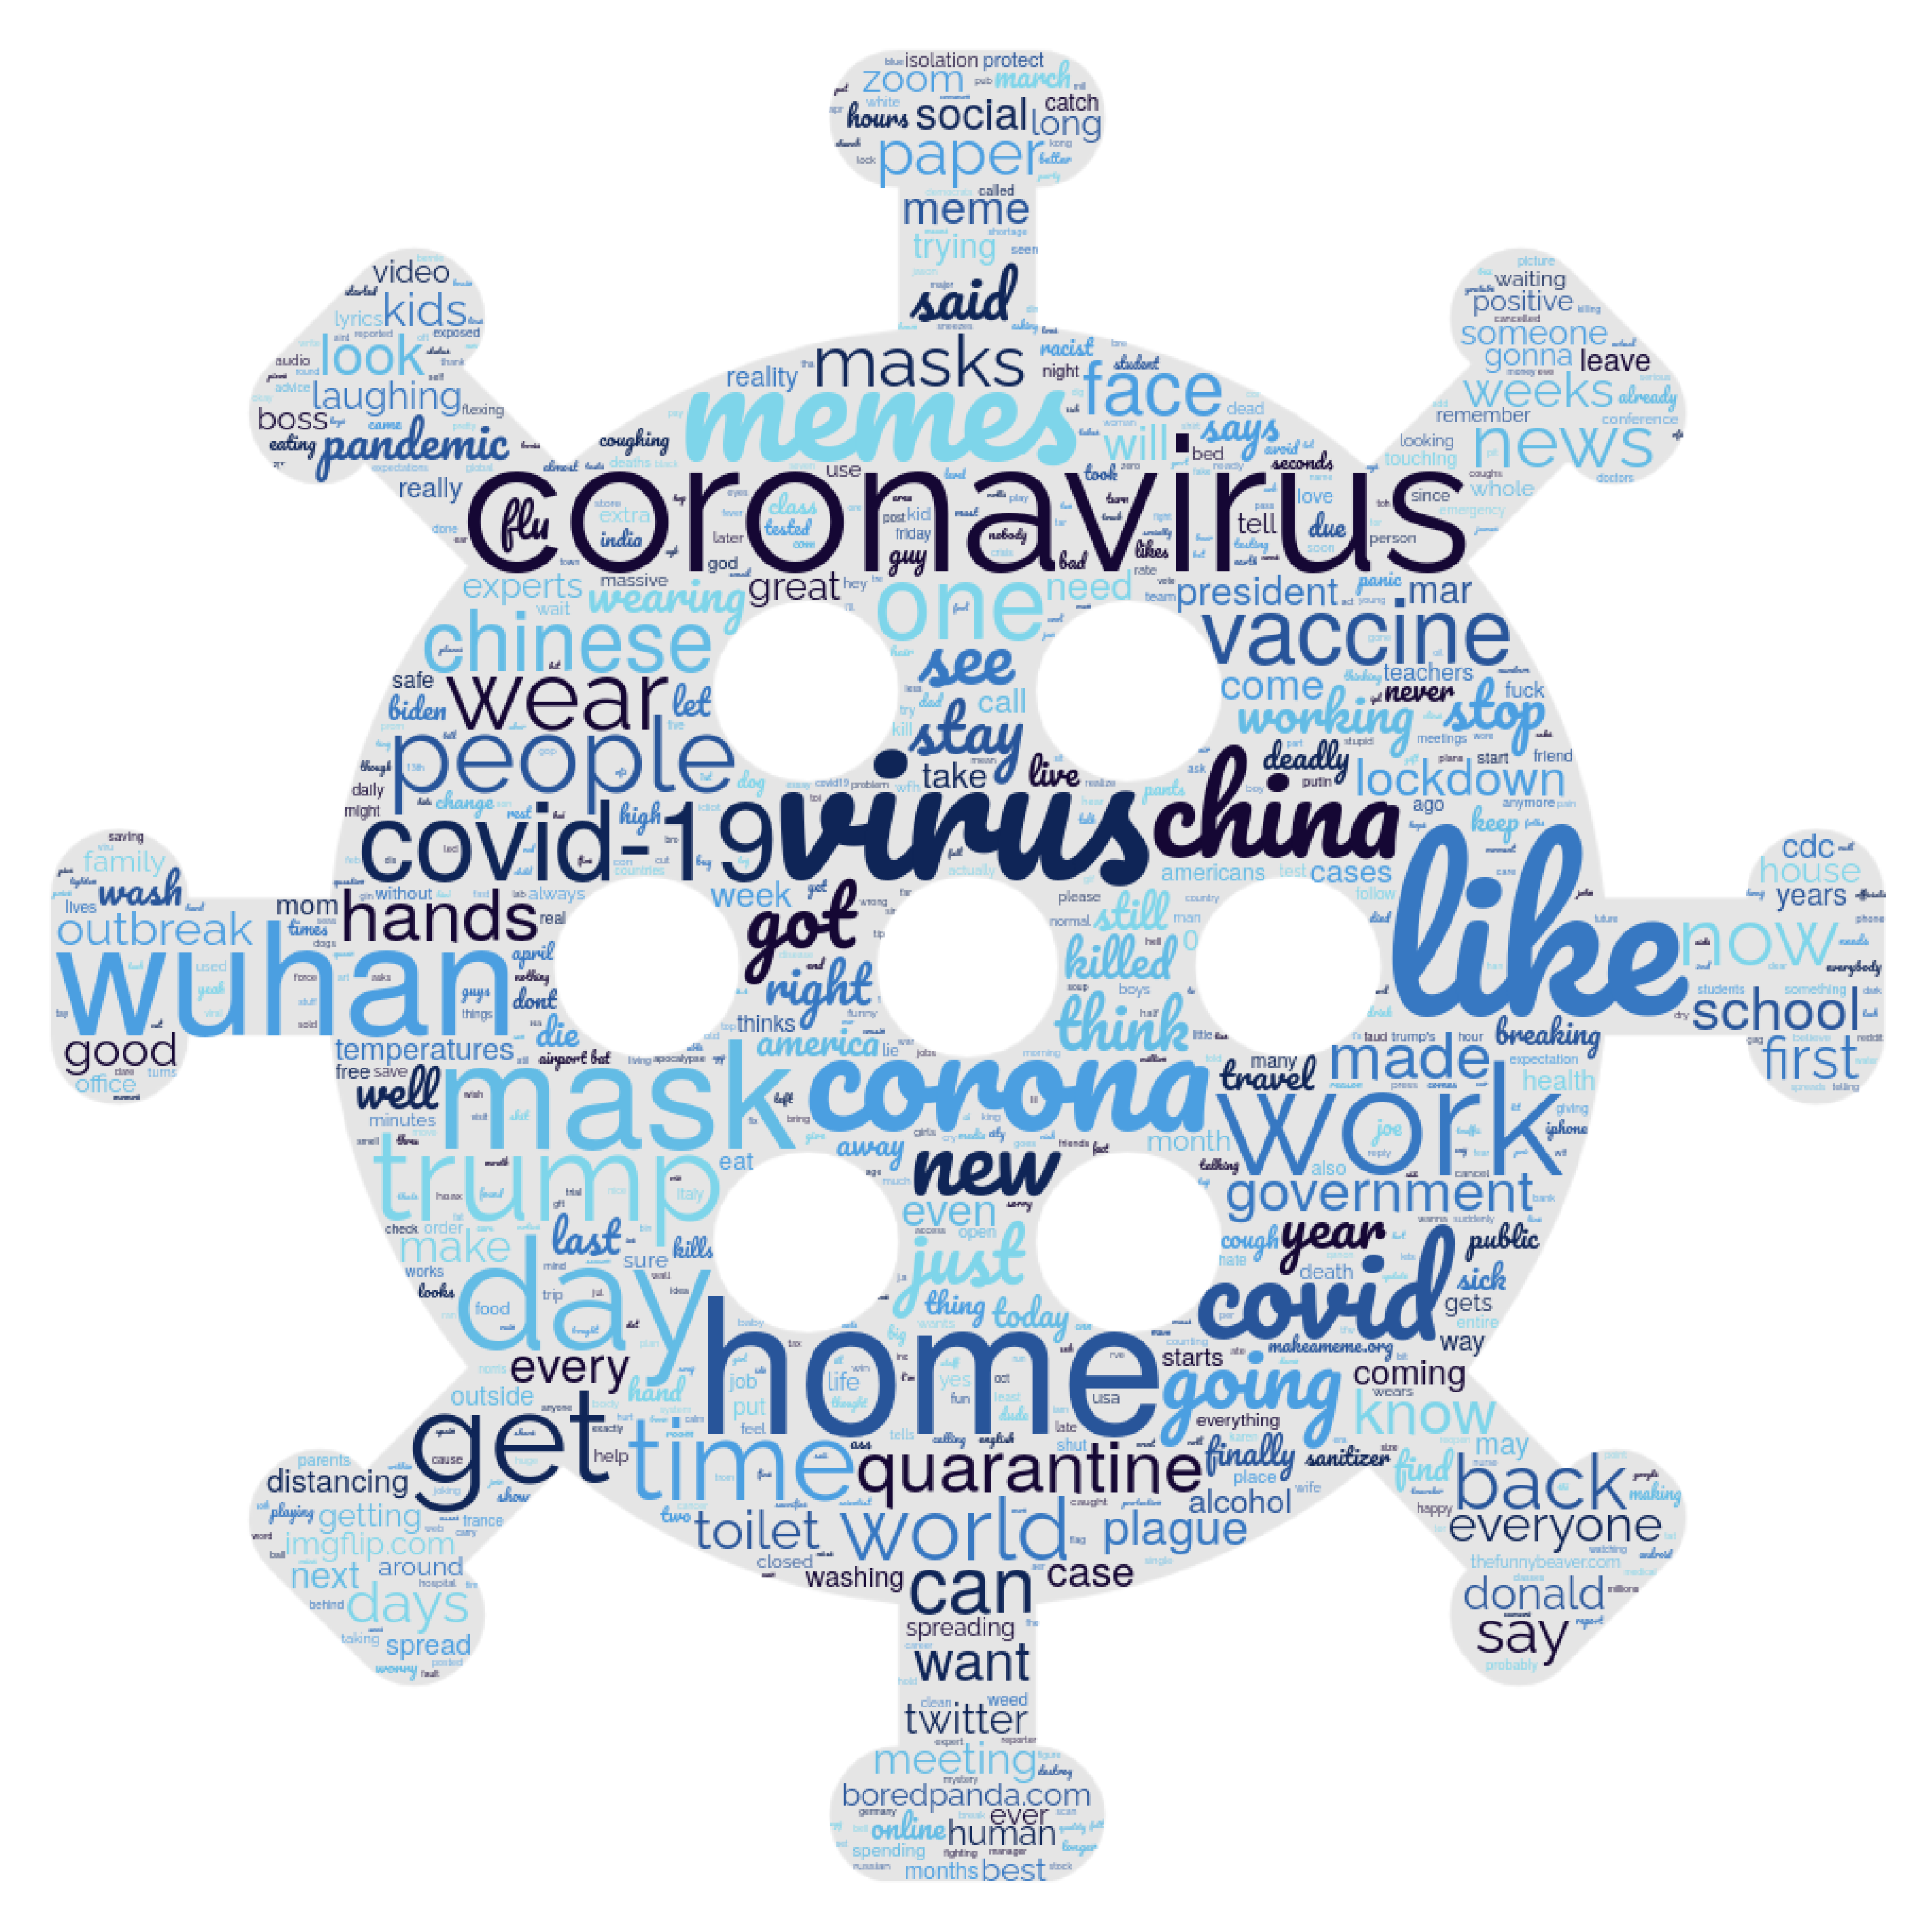
\includegraphics[width=0.45\textwidth]{figures/Data_Stats/wordcloud_covid19a.pdf}}\hspace{0.1mm}
\subfloat[{US Politics}\label{fig:cloud_pol}]{
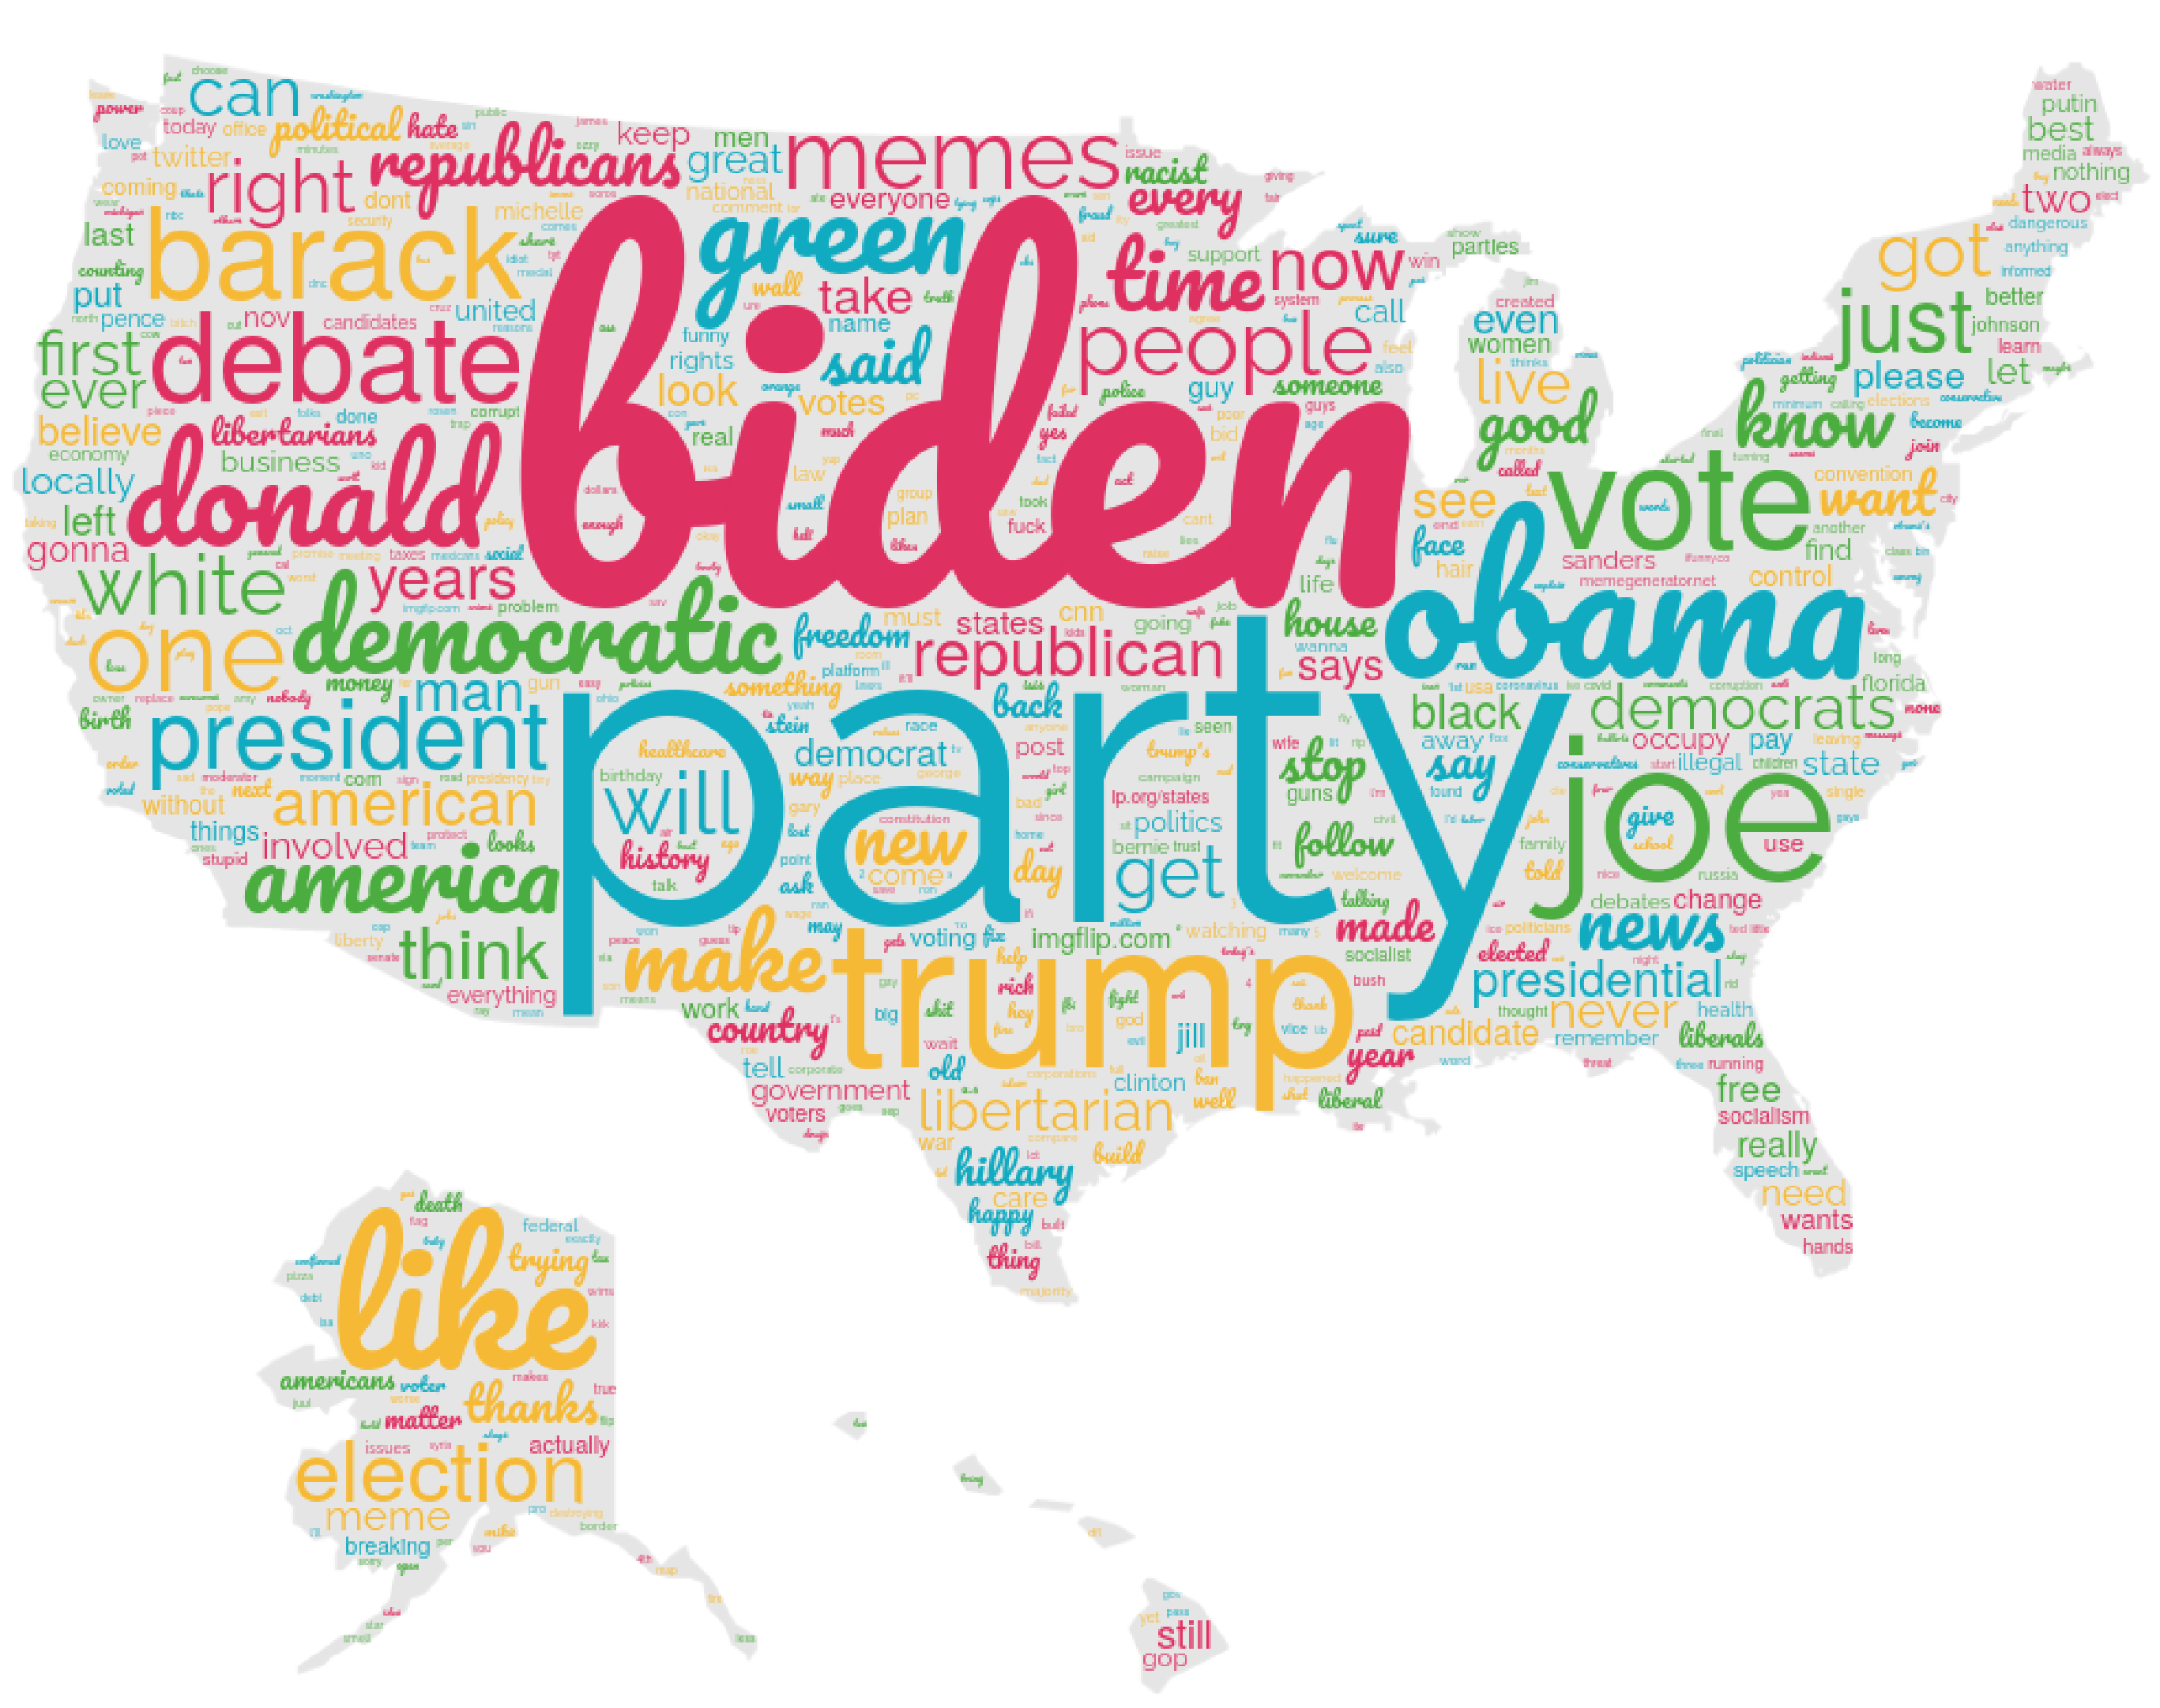
\includegraphics[width=0.45\textwidth]{figures/Data_Stats/wordcloud_uspol2_crop.pdf}}\hspace{0.1mm}
\caption{Word clouds for (a) COVID-19 and (b) US Politics domains in \dataset.}
\label{fig:gen_stat}
\end{figure*}
\section{Dataset Curation}
\label{sec:dataset}
Towards curating a dataset that facilitates the connotative labels: Hero, Villain and Victim, we leverage, and reannotate harmeme\ dataset released in 
\cite{pramanick-etal-2021-momenta-multimodal}, and call this new dataset as \dataset.
% \ ({\bf R}ole {\bf I}dentification of {\bf M}eme {\bf E}ntities). 
\harmeme\ originally consists of $3544$ memes about COVID-19 (C) and $3552$ memes about US Politics (P), annotated for \textit{harmfulness detection} and \textit{target type identification} for harmful memes, with categories  \textit{individuals, organisations, communities, and society}. 
The summary of the statistics of total $3381$ (after filtering-out the noisy memes) and $3552$ memes for COVID-19 and US Politics, respectively, in \dataset\ is presented in Table \ref{tab:dataset_summary}. As a general trend for both the domains (COVID-19 and US Politics), we observe neutral referencing for most of the entities within memes for both the domains (C: $3065$, P: $3242$). For such cases, we assign a fourth category \textit{other}. On the other hand, \textit{villain} has the second-highest referencing of different entities(C: $747$, P: $1641$), followed by \textit{victim} (C: $407$, P: $544$), and finally \textit{hero} (C: $200$, P: $288$). Such a trend reasonably emulates the realistic representation of social media engagement involving memes, mostly humorous with neutral connotations and harmful, by indulging in vilification. Victimisation can also be interpreted as the countering resistance against incessant vilification. Glorification is found to have the weakest voice via memetic discourses observed. This highlights the investigative need to characterise various connotative referencing within memes.


 
% Please add the following required packages to your document preamble:
% \usepackage{multirow}
\if 0
\begin{table}[t!]
\centering
\caption{Statistics of our proposed \dataset\ dataset.}
\label{tab:dataset_summary}
\resizebox{0.5\textwidth}{!}{%
\begin{tabular}{c|c|c|c|c|c|c}
\hline
\multirow{2}{*}{\textbf{Domain}} & \multirow{2}{*}{\textbf{Splits}} &  \multirow{2}{*}{\textbf{\# Samples}} & \multicolumn{4}{c}{\textbf{\# References}} \\
\cline{4-7}
 &  &  & \textbf{Hero} & \textbf{Villain} & \textbf{Victim} & \textbf{Other} \\ \hline
\multirow{4}{*}{\rotatebox[origin=c]{90}{COVID-19}} & Train & 2700 & 163 & 576  & 317 & 2438 \\
                          & Val   & 300  & 19  & 65   & 40  & 268  \\
                          & Test  & 381  & 18  & 106  & 50  & 359  \\ \cline{2-7} 
                          & Total & 3381 & 200 & 747  & 407 & 3065 \\ \hline
\multirow{4}{*}{\rotatebox[origin=c]{90}{Politics}} & Train & 2852 & 230 & 1308 & 441 & 2617 \\
                          & Val   & 350  & 27  & 166  & 58  & 317  \\
                          & Test  & 350  & 31  & 167  & 45  & 308  \\ \cline{2-7} 
                          & Total & 3552 & 288 & 1641 & 544 & 3242 \\ \hline
\end{tabular}}
\end{table}
\fi






% \begin{wrapfigure}[9]{R}{0.25\textwidth}
% \vspace{-22pt}
% \centering
% \includegraphics[width=0.25\textwidth]{figures/Trump_Mask.png}
% % \vspace{-10pt}
% \caption{\label{fig:donald_mask}Edge case}
% \end{wrapfigure}

\subsection{Annotation Details} Since entity role labelling is a reasonably subjective and complex task, we formulated standard guidelines towards the annotation (see Table \ref{tab:annot_table}). Also, three annotators and a consolidator ensured the required alignment of the labels wherever a consensus couldn't be reached. The task required annotators to (i) identify the entities and (ii) assign roles to the entities identified in (i). 

% Since role-labelling in memes is a reasonably subjective annotation process, we assigned three specialised annotators to annotate the entire dataset and one consolidator for resolving the disagreements incurred thereof. The annotators are responsible for identifying entities from each meme and subsequently labelling their roles. 

\paragraph{\bf Identifying Entities.} This step required an annotator to elicit all the candidate entities from a given meme. The entities could be either: \textit{person}, \textit{norp} (nationalities or religious or political group), \textit{facility, organization, geopolitical entity, location} or \textit{product}, amongst few other standard entities as defined by spaCy's label scheme for NER module\footnote{\url{https://spacy.io/models/en\#en_core_web_sm}}. The entities identified pertain prominently to various social, global, political, and economic factors for the `COVID-19' domain like \textit{coronavirus, china, home, wuhan, mask, work}, etc. as can be visualised via the word cloud depicted in Fig. \ref{fig:cloud_covid}. Whereas, for `US Politics', entities like \textit{biden, party, donald, democratic, obama}, etc. are identified (see Fig. \ref{fig:cloud_pol}). An exhaustive list of all possible entities that can be identified was shared with the annotators, along with \textit{resolution remarks} whenever required (see Table \ref{tab:res_table}), to assist with their entity identification. To assess the general agreement amongst annotators, we considered an agreement towards entity identification if at least 2 annotators agreed upon any entity implied within meme. This was normalised by the total meme count, having at least one valid entity assignment by the annotators. This was done independently of the implied role category, as the emphasis is only on entity identification. The highest agreement towards this was $0.98$, which suggests the reliability associated with their collective understanding of the task. We follow a similar approach towards the overall role-wise inter-annotator agreement, which we elaborate on in subsequent paragraphs. 

% This stage follows the identification of all entities explicitly referenced in memes (through either visual or textual expressions). The following is the entity-wise inter-annotator agreement (IAA) formulation -- for each entity in a meme, if at least two (out of three) annotators identify the same, it is a valid agreement. The IAA score is a whopping $0.98$, so we do not elaborate further on the same.

\paragraph{\bf Role Assignment.} In the \textit{first} stage of the annotation process, `dry-run', annotators examined their basic agreement quality for a random subset of $250$ memes. With an initially sub-optimal agreement of $0.50$, $0.35$, $0.14$, and $0.55$, for roles `hero', `villain', `victim', and `other', respectively, we decided to transition to the \textit{second} stage: `completion'. Towards annotating the \textit{complete} set (stage-2), annotators and consolidator were provided with detailed guidelines, along with the basic definition of each role category. The annotation agreement was assessed once after the \textit{completion} stage, and then finally after the \textit{consolidation} stage.

% The annotation ensued in three stages: (i) dry-run, (ii) complete annotation, and (iii) consolidation. As part of the dry-run, annotators annotated a random subset of $250$ memes, assigning the entities the roles of `hero', `villain', `victim', and `other'. This resulted in non-impressive role-wise inter-annotator agreement scores of $0.50$, $0.35$, $0.14$, and $0.55$, respectively. We elaborate on our agreement scoring strategy later. The annotators were then trained by issuing detailed guidelines that included the formal definitions of role categories and the instructions exemplifying the edge scenarios identified as part of dry-run disagreements.   

% Besides including the formal definitions of \textit{hero, villain, victim, and other} role categories, annotation guidelines additionally constituted basic steps to follow, along with the unique set of instructions exemplifying the edge scenarios identified as part of dry-run disagreements.   

% \paragraph{\bf Edge Case.}
% A majority of memes are intended towards projecting harmless mockery towards various sections of society. Such memes do not imply heroes, villains or victims; instead, they serve the purpose of disseminating harmless humour and trivial opinions. Therefore, we do not presume any implications regarding these connotations and categorise them as `other', a fourth \textit{neutral} category, unless expressed otherwise in the meme.
% A depiction of such a scenario can be observed in Fig. \ref{fig:donald_mask}. In this meme, it is unclear if Donald Trump is being vilified for being reluctant to use a mask, or the meme expresses just a benign attempt at mocking his physical appearances with sarcasm. Additionally, since no amount of background information would suffice to facilitate its complete assimilation, it can be categorised as \textit{other}.

% \todo[inline]{Add Total column to the summary table.}

% \paragraph{\bf Annotation Guidelines.}
% Several key points, included as part of the annotation guidelines, are enlisted below: 
% \begin{enumerate}
%     \item The role assessment has to be done while considering the meme author's perspective as a common frame of reference.
%     \item Both visual and textual cues should be primarily considered towards comprehension.
%      \item The meme must be completely assimilated whilst considering any associated background context before assigning the designated roles. 
%     %  As some cases might not be clear halfway through the assessment. 
%     % The conclusion should form the basis for the category assignment.
%     \item Contextual dependency beyond an intelligibility threshold should be designated complex enough to be categorised as either of \textit{hero}, \textit{villain}, or \textit{victim}. It should be categorised as \textit{other} instead.
%     \item The role assessment for an entity needs to factor in a three-point Likert scale of affect: positive, negative and neutral inherently.
%     \item All the visually and linguistically intelligible entities should be considered valid towards role assessment.
%     \item If an entity belongs to multiple categories or can potentially have multiple interpretations, it could be categorised as \textit{other}.
%     \item If there is a quote mentioned, the person quoting should not be categorised as either a \textit{hero}, a \textit{villain} or a \textit{victim} unless connotated explicitly and be categorised as \textit{other}.
% \end{enumerate}
% \vspace{-5mm}
\begin{table}[t!]
    \centering
    \label{tab:iaa}
\resizebox{\columnwidth}{!}{%
\begin{tabular}{c|cc|cc|c}
\multicolumn{6}{c}{} \\
\multicolumn{6}{c}{} \\
\hline
\multirow{2}{*}{\textbf{Roles}} &
  \multicolumn{2}{c|}{\textbf{Covid-19} ($\kappa$)} &
  \multicolumn{2}{c|}{\textbf{US Politics} ($\kappa$)} &
  \multirow{2}{*}{\begin{tabular}[c]{@{}c@{}}\textbf{Stage-3}\\  \textbf{Avg.} ($\kappa$)\end{tabular}} \\ \cline{2-5}
 &
  \multicolumn{1}{c|}{\textbf{Stage-2}} &
  \textbf{Stage-3} &
  \multicolumn{1}{c|}{\textbf{Stage-2}} &
  \textbf{Stage-3} &
   \\ \hline
Hero    & \multicolumn{1}{c|}{0.30} & 0.54 & \multicolumn{1}{c|}{0.36} & 0.51 & 0.53 \\ %\hline
Villain & \multicolumn{1}{c|}{0.31} & 0.55 & \multicolumn{1}{c|}{0.55} & 0.73 & 0.64 \\ %\hline
Victim  & \multicolumn{1}{c|}{0.21} & 0.55 & \multicolumn{1}{c|}{0.24} & 0.43 & 0.49 \\ %\hline
Other   & \multicolumn{1}{c|}{0.58} & 0.68 & \multicolumn{1}{c|}{0.76} & 0.88 & 0.78 \\ \hline
Avg.    & \multicolumn{1}{c|}{0.35} & \textbf{0.58} & \multicolumn{1}{c|}{0.48} & \textbf{0.64} & \textbf{0.61} \\ \hline
\end{tabular}}
\caption{Inter-annotator agreement (IAA) summary for \textit{completed} (Stage-2) and \textit{consolidated} (Stage-3) stages of the annotation process. Average IAA for dry-run (Stage-1, for both COVID-19 and US Politics): $0.50$ (hero), $0.35$ (villain), $0.14$ (victim), and $0.55$ (other).}
\label{tab:iaa}
\end{table}
\subsubsection{Inter-annotator Agreement}
Due to the varying annotation responses and co-referencing for each role, conventional annotation agreement metrics do not suffice in our setup. We consider an agreement for a sample when at least two annotators agree on one of the candidate entities for a particular role. The role-wise agreement is then normalised using the total cases in which at least one valid (non-null) entity was marked. This facilitates role-wise IAA scores, as shown in Table  \ref{tab:iaa}. We denote this formulation via $\kappa$ and express it as follows:
% \begin{array}{cccc}
%      v_{agr} &= \sum_{i=1}^{N}I_{i} & v_{tot} &= \sum_{i=1}^{N}Z_{i}
% \end{array}
\begin{equation}
    v_{agr} = \sum_{i=1}^{N}I_{i};~v_{tot} = \sum_{i=1}^{N}Z_{i}
\end{equation}
where $I$, $Z$, $N$, $v_{agr}$, $v_{tot}$ denote a valid agreement (1 if at least two annotators agree for an entity), valid response (1 if at least one annotator provides a valid entity as a response), total samples in the dataset, total valid agreement and total valid responses, respectively.

\begin{equation}
    \kappa = \frac{v_{agr}}{v_{tot}}
\end{equation}
where $\kappa$ is the final agreement score. 
% \begin{equation}
    
% \end{equation}

The agreement scores after the \textit{completion} stage (stage-2) are $0.35$ and $0.48$ for COVID-19 and US Politics domains, respectively. The consolidation stage (stage-3) facilitated enhancements of $0.23$ and $0.16$ absolute points, respectively, over the scores after stage-2. The summary of inter-annotator agreement is shown in Table \ref{tab:iaa}.
% A significant enhancement in the overall agreement scores is observed after consolidation stage. As can be observed from Table \ref{tab:iaa}, the final \textit{consolidation} was observed to induce an enhancement of $0.23$ and $0.16$ absolute points, over the agreements of $0.35$ and $0.48$, observed after \textit{complete} annotation stage, for COVID-19 and US Politics domains, respectively.


\subsection{Role-wise Analysis of \dataset}

% \begin{figure*}[t!]
% \centering
% \subfloat[{COVID-19}\label{fig:count_covid}]{
% \includegraphics[width=0.45\textwidth]{figures/Data_Stats/donut_COV.pdf}}\hspace{0.1mm}
% \subfloat[{US Politics}\label{fig:count_pol}]{
% \includegraphics[width=0.45\textwidth]{figures/Data_Stats/donut_POL.pdf}}\hspace{0.1mm}
% \caption{Distribution of entities across different datasets.}
% \label{fig:gen_stat}
% \end{figure*}

% \begin{figure*}[t!]
% \centering
% \subfloat[{COVID-19}\label{fig:dist_covid}]{
% \includegraphics[width=0.45\textwidth]{figures/Data_Stats/ent_dist_COVID19.pdf}}\hspace{0.1mm}
% \subfloat[{US Politics}\label{fig:dist_uspol}]{
% \includegraphics[width=0.45\textwidth]{figures/Data_Stats/ent_dist_USPOL.pdf}}\hspace{0.1mm}
% \caption{Distribution of roles of top 10 entities across two datasets.}
% \label{fig:role_dist_harmeme}
% \end{figure*}

The distribution of the amount of referencing of different entities within \dataset,\ suggests a pattern of predominant referencing of particular entities within different contexts of memes. The entities fairly emulate the prevalent trends and discourse themes that social media engagement around the period of dataset collection reflected, which was at the onset of the COVID-19 pandemic and the surrounding political outlook within the United States.   


% Such trends highlight the key figures and real-world topics that dominated memetic communication on social media during the period this dataset was compiled, which coincided with the onset of the global COVID-19 pandemic and contemporary US Politics. 
% On analysing entities that are referenced most within memes, it is observed that entities like  \textit{donald trump and china} are referenced almost equally within vilifying and neutral contexts (see Fig. \ref{fig:dist_covid}). 

We also observe that entities like \textit{Donald Trump} and \textit{China} are referenced almost equally in \textit{COVID-19} memes as \textit{villain} and \textit{other}, and other entities are invariably referenced as \textit{other} via humor, sarcasm, limerick, etc. Whereas for \textit{US Politics}, on one hand, entities like \textit{Donald Trump}, \textit{Democratic Party}, \textit{Republican Party}, and \textit{Democrats} are observed to have similar trend of pre-dominant referencing as roles \textit{villain} and \textit{other}, on the other hand, as a general trend, most of the memes are observed to have atleast one vilified referencing. 



\section{Shared Task Details}
The CONSTRAINT 22 Shared Task on Dissecting the Hero, Villain and the Victim in Memes comprise one comprehensive task as follows - \par
\textbf{Role labeling of memes}: The task is to detect which entities are glorified, vilified or victimised within a meme. The underlying assumption for the frame of reference for adjudicating these roles was employed as meme author's perspective. The shared task's objective is to detect whether an entity referenced within a given meme is being glorified, vilified or victimised.\par

Participants were provided with individual Train and Validation splits of Covid-19 and US Politics memes as discussed in Section \ref{sec:dataset}. The Covid-19 and US Politics memes were combined and shuffled as part of the test set to evaluate participants' submissions on both domains comprehensively. 

\subsection{Evaluation Metrics}
The official evaluation measure for the shared task is the macro-F1 score for the multi-class classification. The evaluation is done at the corpus level and not at the sample (meme) level. We allowed the participants a maximum of 25 submissions, and the best submission was considered for the leader-board.  

\subsection{Task Organisation}
The task was organized on Codalab, an open-source platform widely used to host machine learning and data science competitions. Our competition link\footnote{\url{https://codalab.lisn.upsaclay.fr/competitions/906}} provides all the necessary resources for the participants with archived news, notifications and forum posts communicated during the shared task.

% \paragraph{Development Phase}
% The development phase was started on January 6th. 

% \paragraph{Test Phase}

\begin{table}
\resizebox{\columnwidth}{!}{%
\begin{tabular}{c|c|c|c|c}
    \hline
    \textbf{Rank} & \textbf{System} & \textbf{Precision} & \textbf{Recall} & \textbf{F1} \\\hline
    1 & Logically & 55.76 & 62.73 & 58.67  \\
    2 & c1pher & 53.91 & 57.25 & 55.24 \\
    3 & zhouziming & 54.19 & 55.36 & 54.70 \\
    4 & smontariol & 57.96 & 44.97 & 48.48 \\
    5 & IIITDWD & 25.57 & 23.79 & 23.85 \\
    6 & rabindra.nath & 25.30 & 25.30 & 23.71 \\
    \hline
\end{tabular}
}
\caption{Leader-board summary for shared task.}
\label{tab:results}
\end{table}

% \begin{table}
% \resizebox{\columnwidth}{!}{%
% \begin{tabular}{c|c|c|c|c}
%     \hline
%     Rank & System & Precision & Recall & F1 \\\hline
%     1 & Logically & 55.766 & 62.730 & 58.671  \\
%     2 & c1pher & 53.912 & 57.259 & 55.24 \\
%     3 & zhouziming & 54.194 & 55.364 & 54.707 \\
%     4 & smontariol & 57.968 & 44.972 & 48.483 \\
%     5 & IIITDWD & 25.577 & 23.799 & 23.855 \\
%     6 & rabindra.nath & 25.304 & 25.307 & 23.717 \\
%     \hline
% \end{tabular}
% }
% \caption{Leader-board summary for shared task.}
% \label{tab:results}
% \end{table}
\begin{table*}
\resizebox{\columnwidth}{!}{%
\begin{tabular}{c|c|c|c|c|c|c|c|c|c|c|c|c|c|c|c|c|c}
    \hline
    \bf System & \bf BERT & \bf R-BERT & \bf D-BERT & \bf CLIP & \bf EB7 & \bf OFA & \bf ViLT & \bf ViT & \bf VB & \bf U & \bf O & \bf E-V & \bf SVM & \bf XGB & \bf BF & \bf VADER & \bf W-P \\ \hline
    \bf Logically & & \checkmark & \checkmark & & \checkmark & & \checkmark & & & & & & & &  & & \\ \hline
    \bf c1pher & \checkmark & \checkmark & & & & & & & & & & & \checkmark &  &  & & \\ \hline
    \bf zhouziming & & & & & & & & & \checkmark & \checkmark & \checkmark & \checkmark & \checkmark  & & & \\ \hline
    \bf smontariol &  & & & \checkmark & & \checkmark & & & \checkmark &  &  &  & & \checkmark & & \\ \hline
    \bf IIITDWD  &  & & & & &  & & & &  &  &  &  & & & \checkmark & \checkmark \\ \hline
    \bf rabindra.nath & \checkmark & & &  & & & & \checkmark & &  &  &  & \checkmark & & \checkmark & \\ \hline
    
\end{tabular}
}
\caption{Models used by the participants as part of their system submissions. \textbf{R-BERT:} RoBERTa, \textbf{D-BERT:} DeBERTa, \textbf{EB7:} EfficientNetB7, \textbf{OFA:} Once-for-All, \textbf{ViLT:} Visual and Lanugage Transformer, \textbf{ViT:} Visual Transformer, \textbf{VB:} Visual BERT, \textbf{U:} UNITER, \textbf{O:} OSCAR, \textbf{E-V:} Ernie-Vil, \textbf{SVM:} Support Vector Machines, \textbf{XGB:} XGBoost, \textbf{BF:} Block Fusion and \textbf{W-P:} Wu-Palmer.}
\label{tab:models}
\end{table*}

\section{Participation and Results}
\label{sec:partres}
The total number of participants registered for the competition was 105. We had nine teams submit to the leader-board for the shared task with a competitive 71 attempts to better their submissions overall. There was diversity in each team's approach, and we discuss the same below - 

\begin{itemize}
    \item \textbf{Logically} achieves the best results overall. One of the distinctive approaches that the authors followed is to make use of Celebrity face detection from the input meme images using Giphy's Github\footnote{\url{https://github.com/Giphy/celeb-detection-oss}}. In addition, a sub-image detector using YoloV5\footnote{\url{https://github.com/ultralytics/yolov5}} leverages the bounding boxes for memes with multiple images. This is input to an ensemble model of DeBERTa \citep{he_deberta_2021} + RoBERTa \citep{liu_roberta_2019} + ViLT \citep{kim_vilt_2021} + EfficientNetB7 \citep{tan_efficientnet_2020} with averaging of predictions in the final layer. Though they have incorporated a celebrity detector, the lack of other external knowledge limits their system performance. Their source code is available at \url{https://bitbucket.org/logicallydevs/constraint_2022/src/master/}.
    \item \textbf{c1pher} secures the second-best results. The remarkable system design to note is that they achieve it using just text input features! They formulate after Multiple Choice Question Answering Task (MCQA) using three modules ensemble - twitter-xlm-roberta + COVID-BERT \citep{muller_covid-twitter-bert_2020} + BERT-tweet \citep{nguyen_bertweet_2020}. This is combined with the Sentiment module trained using RoBERTa with the final classification layer comprising Support Vector Machine (SVM). Despite decent scores, a major shortcoming of this approach remains to be the exclusion of meme image features for modeling. 
    %Code - Not available
    \item \textbf{zhouziming} leverages the Visual Commonsense Reasoning (VCR) framework in their multimodal model implementations. With this approach, the authors ensemble VisualBERT \citep{li_visualbert_2019} + UNITER \citep{chen_uniter_2020} + OSCAR \citep{li_oscar_2020} + ERNIE-Vil \citep{yu_ernie-vil_2021} with SVM at the final layer to combine the predictions. To handle the disproportionately large ``other'' class in the dataset, the authors introduce loss-reweighting to reduce the ``other'' class's influence on weight updates. Lack of sufficient external knowledge and position information of OCR text with images in the meme restricts their system performance. Their source code is available at \url{https://github.com/zjl123001/DD-TIG-Constraint}.
    \item \textbf{smontariol} experiments with sampling techniques to handle the data imbalance while discussing six strategies. On top of that, they opt for an ensemble of CLIP \citep{radford_learning_2021} + VisualBERT + OFA \citep{cai_once-for-all_2020} with XGBoost as the final layer for classification. The limitations discussed include errors in OCR (Optical character recognition), entity matching with their corresponding positions in the image, and (or) OCR. Their source code is available at \url{https://github.com/smontariol/mmsrl_constraint}.
    % \item \textbf{amanpriyanshu}
    \item \textbf{IIITDWD} combines a sentiment-based and lexicon-based approach to associate sentiment polarity and roles to each entity. For Sentiment classification, the authors use VADER-Sentiment\footnote{\url{https://pypi.org/project/vaderSentiment/}}. In addition, to associate commonly used words for \emph{hero, villain and victim}, the authors develop a corpus and use Wu-Palmer similarity\footnote{\url{https://arxiv.org/ftp/arxiv/papers/1310/1310.8059.pdf}} scores for the same. It is unclear how this corpus is built and how these two approaches are efficiently combined, obscuring this system's limitation. Their source code is available at  \url{https://github.com/fharookshaik/shared-task_constraint-2022}.
    \item \textbf{rabindra.nath} proposes an approach of BLOCK fusion \citep{ben-younes_block_2019} for combining the image and text embeddings. The authors use a combination of ViT \citep{bobicev-sokolova-2017-inter} and BERT \citep{devlin_bert_2019} for image and text, respectively, followed by SVM as the final layer for classification. The empirical approach limits their system performance despite adding several data augmentation techniques. Their source code is available at \url{https://github.com/robi56/harmful_memes_block_fusion}.
    %Code - Not available
\end{itemize}

The results of each system is presented in Table ~\ref{tab:results}. The macro-F1 scores range between $58.671\%$ to $23.717\%$ with a mean score of $44.108\%$ and median score of $51.59\%$.\par
We consolidate the different model architectures used by the participants in Table \ref{tab:models}. One commonly used architecture is BERT and its variants, whereas SVM has been the preferred final layer for classification by three among the six participants. 




\section{Conclusion}
Understanding and interpreting the connotations behind the entities in a meme is a difficult task. Through this shared task, we introduced the novel task of role labeling of entities in harmful memes as hero, villain, and victim. We curated \dataset, a large-scale meme dataset of around $7000$ memes spanning the domains of COVID-19 and US Politics, each tagged with the hero, villain, and victim entities. The shared task attracted $105$ participants, with $6$ participants submitting the final results. We brought to light a new research direction to analyze the entitles in a meme and encourage further detailed work in this area through this shared task.

% This paper introduced a novel task of identifying the roles of entities in harmful memes and discussed its challenges. We curated \dataset, the first-of-its-kind meme dataset of around $7000$ memes spanning the domains of COVID-19 and US Politics, adroitly tagged with the hero, villain, and victim entities. We further presented numerous unimodal and multimodal baselines to benchmark \dataset. We also developed an extensive set of annotation guidelines and released them for further research. Moreover, we proffered \model, a contextual knowledge enriched multimodal framework that bolsters the multimodal representations with entity-based external knowledge, using a cross-modal attention scheme. \model\ shows noteworthy improvements over the baselines, thus justifying contextual knowledge inclusion. As for future investigations, we plan on conceiving a more symbolic system with graph-based entity linking, commonsense knowledge, and visual concepts.



% \clearpage
% Entries for the entire Anthology, followed by custom entries
\bibliography{anthology,custom}

% \appendix

% \section{Example Appendix}
% \label{sec:appendix}

% This is an appendix.

\end{document}
